% =====================================================================
% TA-IND-01 — Informe Académico Individual:
% análisis crítico de un sistema distribuido real
% Compilar: pdflatex -> biber -> pdflatex -> pdflatex
% =====================================================================
\documentclass[11pt,a4paper]{article}

% ---------- Codificación e idioma ----------
\usepackage[utf8]{inputenc}
\usepackage[T1]{fontenc}
\usepackage[spanish,es-tabla]{babel}
\usepackage{csquotes}

% ---------- Formato académico: Times 11 pt, márgenes 2,54 cm ----------
\usepackage{mathptmx}                 % Times (cuerpo y matemáticas)
\usepackage[margin=2.54cm]{geometry}
\usepackage{microtype}
\usepackage{setspace}
\singlespacing
\setlength{\parindent}{0pt}
\setlength{\parskip}{6pt}
\usepackage{ragged2e}
% (el texto ya sale justificado por defecto en article)

% ---------- Títulos: 16/14/12 pt en negrita, negro ----------
\usepackage{titlesec}
\titleformat{\section}{\bfseries\fontsize{16}{19}\selectfont}{\thesection.}{0.6em}{}
\titleformat{\subsection}{\bfseries\fontsize{14}{17}\selectfont}{\thesubsection.}{0.6em}{}
\titleformat{\subsubsection}{\bfseries\fontsize{12}{14}\selectfont}{\thesubsubsection.}{0.6em}{}
\titlespacing*{\section}{0pt}{14pt}{6pt}
\titlespacing*{\subsection}{0pt}{12pt}{4pt}
\titlespacing*{\subsubsection}{0pt}{10pt}{3pt}

% ---------- Número de página abajo a la derecha ----------
\usepackage{fancyhdr}
\pagestyle{fancy}
\fancyhf{}
\fancyfoot[R]{\thepage}
\renewcommand{\headrulewidth}{0pt}
\renewcommand{\footrulewidth}{0pt}

% ---------- Figuras, tablas y código ----------
\usepackage{graphicx}
\usepackage{float}
\usepackage{booktabs}
\usepackage{tabularx}
\usepackage{array}
\usepackage{caption}
\captionsetup{font=small,labelfont=bf}
\usepackage{xcolor}
\usepackage{tikz}
\usetikzlibrary{arrows.meta,positioning,shapes.geometric,fit,calc,babel}
\usepackage{listings}
\lstset{
  basicstyle=\ttfamily\small,
  breaklines=true,
  frame=single,
  columns=fullflexible,
  keepspaces=true,
  showstringspaces=false,
  inputencoding=utf8,
  extendedchars=true,
  literate={á}{{\'a}}1 {é}{{\'e}}1 {í}{{\'i}}1 {ó}{{\'o}}1 {ú}{{\'u}}1 {ñ}{{\~n}}1
           {Á}{{\'A}}1 {É}{{\'E}}1 {Í}{{\'I}}1 {Ó}{{\'O}}1 {Ú}{{\'U}}1 {Ñ}{{\~N}}1
}

% ---------- Referencias IEEE con biblatex + biber ----------
\usepackage[backend=biber,style=ieee,sorting=none]{biblatex}
\addbibresource{Referencias/referencias.bib}

% ---------- Enlaces (va casi al final) ----------
\usepackage[hidelinks]{hyperref}

% =====================================================================
% Macros del documento
% =====================================================================
\newcommand{\sistemaA}{CockroachDB}      % sistema principal
\newcommand{\sistemaB}{Apache Cassandra} % sistema comparado

% Modo borrador: los avisos \pendiente{} se ven en rojo.
% Para la versión final cambia \borradortrue por \borradorfalse.
\newif\ifborrador
\borradortrue
\newcommand{\pendiente}[1]{\ifborrador\textcolor{red}{[PENDIENTE: #1]}\fi}

% Marcador de figura/captura (se reemplaza por \includegraphics al tenerla)
\newcommand{\marcador}[2]{%
  \fbox{\parbox[c][#2][c]{0.9\textwidth}{\centering\small #1}}}

% =====================================================================
% Datos de la carátula
% =====================================================================
\newcommand{\universidad}{Universidad Técnica Estatal de Quevedo}
\newcommand{\facultad}{Facultad de Ciencias de la Ingeniería}
\newcommand{\carrera}{Ingeniería de Software}
\newcommand{\asignatura}{Aplicaciones Distribuidas}
\newcommand{\codigoactividad}{TA-IND-01}
\newcommand{\estudiante}{Toaquiza Zambrano Belinda Betzabeth}
\newcommand{\paralelo}{A}
\newcommand{\titulodoc}{Análisis crítico de \sistemaA{} frente a \sistemaB{}}

\begin{document}

% =====================================================================
% CARÁTULA (sin numeración)
% =====================================================================
\begin{titlepage}
  \thispagestyle{empty}
  \centering
  {\Large\bfseries \universidad\par}
  \vspace{0.4cm}
  {\large \facultad\par}
  \vspace{0.2cm}
  {\large Carrera: \carrera\par}
  \vspace{2.2cm}
  {\large Asignatura: \asignatura\par}
  \vspace{0.2cm}
  {\large Código de la actividad: \codigoactividad\par}
  \vspace{1.6cm}
  {\LARGE\bfseries Informe Académico Individual:\\[0.3cm] \titulodoc\par}
  \vspace{2.2cm}
  {\large Estudiante: \estudiante\par}
  \vspace{0.2cm}
  {\large Paralelo: \paralelo\par}
  \vspace{0.2cm}
  {\large Fecha: \today\par}
  \vspace{0.6cm}
  \vfill
\end{titlepage}
\setcounter{page}{1}

% =====================================================================
% RESUMEN (150 a 200 palabras)
% =====================================================================
\section*{Resumen}
\pendiente{Escribe entre 150 y 200 palabras: sistema analizado (\sistemaA), enfoque
(comparación con \sistemaB, conceptos de la Unidad~1, experimento propio) y
conclusiones principales. Redáctalo al final, cuando ya tengas los resultados.}

\medskip
\noindent\textbf{Palabras clave:} \pendiente{4 a 6 palabras clave}.

% =====================================================================
\section{Introducción}
% =====================================================================
% - Qué problema resuelve el sistema
% - Quién lo usa y a qué escala opera
% - Por qué lo elegiste
% - Objetivo del informe y cómo se organiza el documento
\pendiente{Problema que resuelve \sistemaA, quién lo usa, escala de operación,
motivo de la elección y organización del informe.}

% =====================================================================
\section{Arquitectura del sistema}
% =====================================================================
% - Componentes y cómo se comunican
% - Diagrama de arquitectura propio (draw.io o TikZ) y su evolución desde
%   el esquema a mano (Anexo A)
La aplicación cliente envía consultas a un nodo de CockroachDB mediante un controlador compatible con PostgreSQL. La capa SQL analiza y ejecuta las consultas, mientras que la capa de transacciones coordina las operaciones de lectura y escritura. La capa de distribución localiza los rangos de claves y dirige cada operación a las réplicas correspondientes, como se describe en la arquitectura del sistema \cite{cockroachlabsArchitecture}. En el ejemplo del diagrama, la réplica que coordina la escritura es el líder Raft y se comunica con las otras dos réplicas. La escritura se confirma al alcanzar el quórum requerido, es decir, al replicarse en al menos dos de los tres nodos \cite{cockroachlabsReplication}. Finalmente, cada nodo conserva los datos en su almacenamiento local Pebble \cite{cockroachlabsStorage}.

\begin{figure}[H]
  \centering
  \resizebox{\textwidth}{!}{% Diagrama de arquitectura de CockroachDB (TikZ) — se incluye con \input desde main.tex
% Requiere en el preámbulo: tikz con las bibliotecas arrows.meta, positioning, fit y calc.
\begin{tikzpicture}[
    font=\footnotesize,
    >=Stealth,
    cliente/.style={draw=black, fill=gray!12, rounded corners=2pt, text width=6.1cm,
                    minimum height=0.9cm, inner sep=4pt, align=center},
    capa/.style={draw=blue!60!black, fill=blue!8, rounded corners=2pt, text width=6.1cm,
                 minimum height=1.05cm, inner sep=4pt, align=left},
    capaR/.style={draw=green!40!black, fill=green!10, rounded corners=2pt, text width=6.1cm,
                  minimum height=1.05cm, inner sep=4pt, align=left},
    nodo/.style={draw=black!70, dashed, rounded corners=3pt, minimum width=7.2cm,
                 minimum height=2.1cm},
    rep/.style={draw=green!40!black, fill=green!10, rounded corners=2pt, text width=3.2cm,
                minimum height=1.1cm, inner sep=3pt, align=center},
    peb/.style={draw=green!40!black, fill=green!10, rounded corners=2pt, text width=1.9cm,
                minimum height=1.1cm, inner sep=3pt, align=center},
    rango/.style={draw=black!70, fill=gray!8, rounded corners=2pt, minimum width=7.2cm,
                  minimum height=0.6cm, inner sep=3pt, align=center},
    flecha/.style={->, thick},
    raft/.style={<->, thick, dashed, draw=orange!80!black},
    etiq/.style={font=\scriptsize, align=left, inner sep=2pt},
    titulo/.style={font=\footnotesize\bfseries, anchor=west}
]
% ---------- Cliente ----------
\node[cliente] (cli) at (0,0) {\textbf{Aplicación cliente}\\ Controlador compatible con PostgreSQL};

% ---------- Panel A: capas lógicas ----------
\node[capa, below=1.5cm of cli] (sql) {\textbf{SQL} (nodo de entrada)\\ Analiza, optimiza y ejecuta consultas.};
\node[capa, below=0.9cm of sql] (trx) {\textbf{Transacciones}\\ Coordina operaciones y confirmación atómica.};
\node[capa, below=0.9cm of trx] (dis) {\textbf{Distribución}\\ Localiza rangos y enruta solicitudes.};
\node[capaR, below=0.9cm of dis] (rpl) {\textbf{Replicación}\\ Coordina réplicas y consenso Raft por rango.};
\node[capaR, below=0.9cm of rpl] (alm) {\textbf{Almacenamiento}\\ Pebble conserva las versiones de los datos.};

\node[titulo] (hA) at ([xshift=-3.05cm,yshift=-0.6cm]cli.south) {A. Capas lógicas};
\node[titulo] (hB) at ([xshift=5.4cm,yshift=-0.6cm]cli.south) {B. Un rango replicado entre nodos (ejemplo)};

\draw[flecha] ([xshift=1.8cm]cli.south) -- ([xshift=1.8cm]sql.north)
  node[midway, right, etiq, text width=3.1cm] {Envía SQL por el protocolo PostgreSQL};
\draw[flecha] ([xshift=-1.8cm]sql.south) -- ([xshift=-1.8cm]trx.north)
  node[midway, right, etiq, text width=4.0cm] {Solicita operaciones clave--valor};
\draw[flecha] ([xshift=-1.8cm]trx.south) -- ([xshift=-1.8cm]dis.north)
  node[midway, right, etiq, text width=4.0cm] {Envía operaciones clave--valor};
\draw[flecha] ([xshift=-1.8cm]dis.south) -- ([xshift=-1.8cm]rpl.north)
  node[midway, right, etiq, text width=4.7cm] {Dirige la escritura al titular de la concesión};
\draw[flecha] ([xshift=-1.8cm]rpl.south) -- ([xshift=-1.8cm]alm.north)
  node[midway, right, etiq, text width=4.7cm] {Aplica cambios confirmados en cada réplica};

% ---------- Panel B: un rango replicado en tres nodos ----------
\node[nodo] (n2) at ([xshift=9cm,yshift=0.2cm]rpl.center) {};
\node[nodo, above=0.8cm of n2] (n1) {};
\node[nodo, below=0.8cm of n2] (n3) {};
\node[rango, above=0.35cm of n1] (rng) {\textbf{Rango R} = intervalo contiguo de claves};

\foreach \n/\t in {n1/{Nodo 1 (roach1)}, n2/{Nodo 2 (roach2)}, n3/{Nodo 3 (roach3)}}{
  \node[font=\scriptsize\bfseries, anchor=north west] at ([xshift=0.1cm,yshift=-0.05cm]\n.north west) {\t};
}

\node[rep] (r1) at ([xshift=-1.2cm,yshift=-0.2cm]n1.center) {Réplica votante de R\\ \textit{Seguidora}};
\node[rep] (r2) at ([xshift=-1.2cm,yshift=-0.2cm]n2.center) {Réplica votante de R\\ \textit{Líder Raft y leaseholder}};
\node[rep] (r3) at ([xshift=-1.2cm,yshift=-0.2cm]n3.center) {Réplica votante de R\\ \textit{Seguidora}};
\node[peb] (p1) at ([xshift=2.5cm,yshift=-0.2cm]n1.center) {Almacén Pebble};
\node[peb] (p2) at ([xshift=2.5cm,yshift=-0.2cm]n2.center) {Almacén Pebble};
\node[peb] (p3) at ([xshift=2.5cm,yshift=-0.2cm]n3.center) {Almacén Pebble};

\foreach \r/\p in {r1/p1, r2/p2, r3/p3}{
  \draw[flecha] (\r.east) -- (\p.west) node[midway, above, etiq] {Persiste};
}

% Comunicación Raft entre réplicas
\draw[raft] (r1.south) -- (r2.north) node[midway, right, etiq] {Raft};
\draw[raft] (r2.south) -- (r3.north) node[midway, right, etiq] {Raft};

% De la capa de replicación al líder del rango
\draw[flecha] (rpl.east) -- (r2.west);

% ---------- Recuadro del clúster ----------
\node[draw=black, dashed, rounded corners=6pt, inner sep=0.4cm,
      fit=(hA)(hB)(sql)(alm)(rng)(n1)(n3),
      label={[font=\scriptsize\bfseries, anchor=south east]north east:CLÚSTER COCKROACHDB}] (clu) {};

% ---------- Leyenda ----------
\node[etiq, anchor=north west, text width=15cm] at ([yshift=-0.45cm]clu.south west)
  {\textbf{Leyenda:} flecha continua = solicitud o aplicación local; flecha discontinua naranja = comunicación Raft;
   cajas azules = procesamiento y enrutamiento; cajas verdes = replicación y almacenamiento.
   Los roles de Raft se asignan por rango; el líder mostrado es un ejemplo.};
\end{tikzpicture}
}
  \caption{Arquitectura lógica de \sistemaA{} y réplica de un rango en el clúster de tres nodos del experimento (elaboración propia).}
  \label{fig:arquitectura}
\end{figure}

El esquema preliminar mostraba las cinco capas de CockroachDB y un ejemplo de un rango replicado en tres nodos. La versión final amplió esa vista al detallar la función de cada capa y el recorrido de una solicitud desde la aplicación cliente hasta el almacenamiento. También distinguió la réplica líder de las seguidoras y mostró cómo se comunican mediante Raft, cuántas réplicas se necesitan para confirmar una escritura y cómo se guardan los cambios en Pebble en cada nodo.

% =====================================================================
\section{Análisis con los conceptos de la Unidad 1}
% =====================================================================

\subsection{Transparencias de distribución}

La transparencia de distribución describe cuánto puede usar una aplicación los datos sin tener que conocer su ubicación física, el número de réplicas o los cambios internos del clúster. En ambos motores hay transparencias parciales: la interfaz simplifica el acceso, pero las decisiones sobre consistencia, disponibilidad y recuperación siguen siendo visibles para quien opera o programa el sistema.

\paragraph{Acceso.} CockroachDB ofrece una interfaz SQL compatible con el protocolo de red de PostgreSQL; traduce las consultas en solicitudes sobre su almacenamiento distribuido. Cassandra expone CQL mediante su protocolo binario nativo. En los dos casos, el usuario trabaja con una interfaz lógica sin enviar manualmente cada consulta a todas las réplicas \cite{cockroachlabsArchitecture,cockroachlabsDeveloperBasics,apacheCassandraNative}.

\paragraph{Ubicación.} Ambos sistemas ocultan en gran medida dónde reside cada dato. CockroachDB divide el espacio de claves en rangos y distribuye el encaminamiento entre los nodos. Cassandra calcula el token de la clave de partición y entrega la solicitud a las réplicas pertinentes; cualquier nodo puede actuar como coordinador. La ubicación física no forma parte de la consulta normal, aunque sí puede ser relevante para la configuración y la observabilidad \cite{cockroachlabsArchitecture,apacheCassandraDynamo}.

\paragraph{Migración.} La ubicación lógica también permanece separada de la consulta cuando cambian las réplicas. CockroachDB puede reequilibrar rangos entre nodos; Cassandra distribuye tokens en el anillo y permite añadir, mover o retirar nodos. Esta transparencia es operativa, no absoluta: el cambio de topología requiere configuración y puede involucrar movimiento de datos, carga de red y tareas de mantenimiento \cite{cockroachlabsReplication,apacheCassandraDynamo}.

\paragraph{Reubicación.} La ocultación de una transferencia mientras hay carga es parcial. CockroachDB describe la transferencia de instantáneas y la puesta al día de réplicas durante el rebalanceo. En Cassandra, los cambios del anillo y la reparación pueden transferir datos entre nodos. Las fuentes describen estos mecanismos, pero no garantizan que toda consulta en curso termine sin demora o reintento; esa continuidad tampoco se midió en esta práctica \cite{cockroachlabsReplication,apacheCassandraDynamo,apacheCassandraRepair}.

\paragraph{Replicación.} CockroachDB administra réplicas de rangos mediante Raft y el cliente no selecciona los nodos que deben confirmar una escritura. Cassandra replica cada partición según la estrategia del espacio de claves, pero expone al cliente los niveles de consistencia (\texttt{ONE}, \texttt{QUORUM}, \texttt{ALL}, entre otros), que fijan cuántas respuestas espera el coordinador. Por eso Cassandra automatiza la copia de datos, aunque deja visible una parte mayor de la política de lectura y escritura \cite{cockroachlabsReplication,apacheCassandraDynamo}.

\paragraph{Concurrencia.} CockroachDB aplica aislamiento \texttt{SERIALIZABLE} por defecto: el efecto de transacciones concurrentes debe corresponder a algún orden serial. La contención puede provocar reintentos y, si no se resuelve automáticamente, un error visible para la aplicación. Cassandra resuelve mutaciones ordinarias concurrentes por marcas de tiempo y regla de último escrito; no ofrece por ello una transacción serializable global entre particiones. Para operaciones condicionales de una partición ofrece transacciones ligeras basadas en Paxos. Así, en los dos motores la aplicación puede tener que manejar contención o elegir una garantía concreta \cite{cockroachlabsDeveloperBasics,apacheCassandraDynamo,apacheCassandraGuarantees}.

\paragraph{Fallos.} La abstracción también es parcial. CockroachDB puede seguir atendiendo operaciones que conservan mayoría de votantes para el rango, pero puede rechazar una lectura actual o una escritura si falta quórum; también puede perderse la conexión al nodo usado por el cliente. Cassandra deja que el coordinador atienda según el nivel elegido, por lo que una operación con \texttt{ONE} puede responder cuando niveles mayores no alcanzan sus réplicas requeridas. Los errores de disponibilidad, los tiempos de espera y los reintentos no quedan ocultos por completo \cite{cockroachlabsReplication,apacheCassandraDynamo}.

\subsection{CAP y PACELC}

CAP y PACELC describen compromisos bajo supuestos concretos, no una etiqueta independiente de la operación. En lo que sigue, la clasificación se limita a lecturas actuales y escrituras ordinarias sobre datos con tres réplicas; las conclusiones empíricas se restringen a las operaciones registradas en los experimentos \cite{cockroachlabsReplication,apacheCassandraDynamo,apacheCassandraGuarantees}.

Durante una partición de red, CockroachDB prioriza mantener la consistencia de las operaciones que confirma: Raft exige mayoría de las réplicas del rango. En una disposición de tres réplicas, el lado con dos puede avanzar y el lado con una no puede confirmar una escritura que requiere quórum. Por ello, para estas operaciones CockroachDB presenta el perfil CP: tolera la partición, pero sacrifica disponibilidad en la minoría. En Cassandra el compromiso depende del nivel por operación. La documentación describe su orientación AP; en la práctica, \texttt{ONE} puede responder en cada lado si cada uno alcanza una réplica, mientras que \texttt{QUORUM} solo alcanza el mínimo en la mayoría y \texttt{ALL} requiere las tres. Con niveles más exigentes, Cassandra también sacrifica disponibilidad en el lado que no reúne las respuestas \cite{cockroachlabsReplication,apacheCassandraDynamo,apacheCassandraGuarantees}.

Los ensayos concuerdan con ese contraste, dentro del alcance de las salidas observadas. Las salidas propias constan en \texttt{experimento/comandos.md}, apartados de E1 y E2. En E1, CockroachDB leyó y escribió con un nodo detenido; al detener dos, la consulta devolvió \texttt{replica unavailable}. En E2, el lado mayoritario confirmó la fila 31 y la lectura actual desde \texttt{roach3} aislado falló con \texttt{lost quorum}; el \texttt{INSERT} de la fila 32 quedó sin respuesta visible, así que no se afirma si se confirmó. En Cassandra, la partición 2+1 mostró que \texttt{ONE} completó lecturas y escrituras en ambos lados; \texttt{QUORUM} solo en el lado con dos réplicas; y \texttt{ALL} falló en ese lado y no se probó en el aislado. Tras reconectar, \texttt{ALL} devolvió las filas 21, 23 y 24. Como se usaron claves distintas, la prueba no demuestra cómo se resolverían escrituras concurrentes sobre la misma clave \cite{cockroachlabsReplication,apacheCassandraDynamo}.

PACELC añade la pregunta del comportamiento sin partición: consistencia o menor latencia. Para operaciones actuales, CockroachDB mantiene coordinación de consenso y confirmación por mayoría, lo que puede añadir viajes de red; ofrece lecturas históricas de seguidores cuando se acepta menor frescura. El trabajo de VanBenschoten et al. estudia configuraciones de localidad y lecturas locales consistentes en despliegues multirregión; sus resultados explican una optimización posible, pero no predicen la latencia de este clúster local. La inferencia para las operaciones actuales de esta práctica es un perfil PC/EC: ante partición conserva consistencia en la mayoría y, aun sin partición, conserva consistencia mediante coordinación \cite{cockroachlabsReplication,cockroachlabsFollowerReads,vanbenschoten2022multiregion}.

Cassandra permite escoger cuánto espera el coordinador. \texttt{ONE} exige menos respuestas y puede favorecer menor espera; \texttt{QUORUM} y \texttt{ALL} exigen más confirmaciones y restringen las operaciones que pueden responder. Por ello, su perfil sin partición no es único: el nivel elegido mueve el compromiso hacia latencia o consistencia. Ferreira et al. compararon niveles de consistencia en Cassandra y otros motores en despliegues de nube, y hallaron diferencias de rendimiento asociadas a la configuración; da Silva y Lima evaluaron sistemas en un clúster de placas de bajo consumo. Nejati SharifAldin y Nayebi Pour compararon los niveles nativos con un middleware causal externo. Estos estudios usan cargas y topologías distintas y respaldan el compromiso cualitativo, no una predicción numérica para Docker. En la práctica no se midió latencia; por tanto, la clasificación PL/EL para \texttt{ONE} y PC/EC para niveles de quórum se presenta como inferencia documental y no como resultado de rendimiento del experimento \cite{ferreira2024consistency,silva2023lowpower,nejati2026cassandra,apacheCassandraDynamo}.

\subsection{Modelos de comunicación}

CockroachDB combina el modelo cliente-servidor hacia la aplicación con coordinación distribuida entre nodos. El cliente envía SQL por el protocolo PostgreSQL a un nodo; internamente, los nodos participantes coordinan transacciones y replicación por rangos mediante Raft. La llamada del cliente es síncrona en el sentido de que espera éxito o error de la operación; la escritura no se confirma antes de obtener el quórum requerido. La replicación, el rebalanceo y la actualización de réplicas ocurren mediante intercambios de red entre nodos. El artículo de Kettaneh et al. describe el mecanismo Leader Leases y su detector distribuido de fallos, mientras el documento de multirregión analiza el efecto de la localidad en las transacciones. Esta descripción es arquitectónica; las capturas de la práctica no exponen los mensajes internos ni su temporización \cite{cockroachlabsDeveloperBasics,cockroachlabsArchitecture,cockroachlabsReplication,kettaneh2026leaderleases,vanbenschoten2022multiregion}.

Cassandra también recibe solicitudes de clientes en un modelo cliente-servidor, pero su clúster opera entre pares: un nodo accesible puede coordinar cada petición y distribuirla a las réplicas. El protocolo nativo transporta mensajes CQL desde el cliente; entre nodos se usa mensajería internodo, y gossip intercambia información de membresía y estado. La respuesta al cliente es síncrona respecto al nivel CQL seleccionado: el coordinador espera el número requerido de respuestas. En paralelo, gossip, hinted handoff y reparación participan en la propagación o convergencia posterior, por lo que el sistema combina comunicación de petición-respuesta con trabajo de fondo asíncrono \cite{apacheCassandraArchitecture,apacheCassandraNative,apacheCassandraMessaging,apacheCassandraDynamo,apacheCassandraRepair}.

\subsection{Tolerancia a fallos}

Con tres votantes para un rango, CockroachDB puede tolerar la pérdida de uno mientras los otros dos se comunican. Si se pierde la mayoría, no confirma nuevas escrituras de ese rango; otras partes del clúster pueden seguir funcionando si conservan sus propios quórums. Raft mantiene el registro replicado y el sistema puede transferir liderazgo y concesiones después de detectar que un nodo no está disponible. El artículo de Kettaneh et al. describe Leader Leases con una detección de vitalidad entre nodos. Como la práctica no inspeccionó métricas internas ni el algoritmo exacto de detección activo, los resultados externos no permiten verificar ese mecanismo directamente \cite{cockroachlabsReplication,kettaneh2026leaderleases}.

En E1, con \texttt{roach2} detenido, CockroachDB mantuvo lectura y escritura; con \texttt{roach2} y \texttt{roach3} detenidos, la consulta no alcanzó quórum. Al iniciar los contenedores, el servicio SQL volvió a responder y las filas confirmadas siguieron disponibles. Sin embargo, \texttt{node status} mostró un estado anómalo de \texttt{roach1} hasta que se reinició; la causa de ese estado no quedó establecida. En E2, con \texttt{roach3} desconectado de la red pero aún encendido, la escritura desde la mayoría funcionó y la lectura actual desde el nodo aislado devolvió \texttt{lost quorum}. Ese escenario comprueba una partición de comunicación, distinta de detener el proceso \cite{cockroachlabsReplication}.

Cassandra detecta disponibilidad de pares a partir de heartbeats y gossip. Si una réplica no está disponible, el coordinador puede conservar una mutación pendiente mediante hinted handoff; ese mecanismo es de mejor esfuerzo. La reparación anti-entropía compara rangos con árboles de Merkle y transmite diferencias, y requiere ejecución operativa con \texttt{nodetool repair}. En E1, con RF=3, \texttt{ONE} y \texttt{QUORUM} funcionaron tras detener un nodo, mientras \texttt{ALL} falló; con dos nodos detenidos, solo \texttt{ONE} completó la lectura y la escritura comprobada. Tras iniciar nodos, el estado llegó a tres \texttt{UN} y \texttt{ALL} leyó las filas confirmadas. En E2, los tres nodos volvieron a \texttt{UN}, pero las consultas posteriores no verifican por sí mismas si se usaron hints o repair; el mecanismo exacto de convergencia quedó sin medir \cite{apacheCassandraDynamo,apacheCassandraRepair,apacheCassandraGuarantees}.

Como caso operativo real, Discord describió que su clúster Cassandra de mensajes llegó a 177 nodos y trillones de mensajes, con latencia impredecible, alta carga de mantenimiento y degradación en cascada asociada a particiones calientes y consultas con consistencia de quórum. La publicación relata una degradación de rendimiento y operación, no una caída total del servicio ni una falla de consenso. El caso muestra que replicación y disponibilidad no evitan problemas producidos por patrones de acceso sesgados y carga; no permite trasladar sus magnitudes a esta práctica \cite{discord2023cassandra}. El análisis de latencia permanece cualitativo porque en los experimentos no se registraron mediciones temporales comparables.

\section{Experimentación propia}
% =====================================================================
% Evidencias de autoría 1 y 2: capturas de ejecución real y experimento propio.
% Comandos y resultados completos van en /experimento del repositorio.

\subsection{Entorno y justificación}
\pendiente{Cómo levantaste el sistema (por ejemplo, Docker), versión y por qué
elegiste ese entorno.}

\subsection{Procedimiento}
\pendiente{Describe el experimento y el concepto de la Unidad~1 que ilustra.}

\begin{lstlisting}[caption={Comandos usados en el experimento (ejemplo de formato).},label={lst:comandos}]
# Reemplaza este bloque por tus comandos reales.
# El archivo completo debe estar en experimento/ del repositorio.
\end{lstlisting}

\subsection{Resultados}
\begin{figure}[H]
  \centering
  % \includegraphics[width=0.9\textwidth]{capturas/captura-01.png}
  \marcador{Captura 1: con tu usuario en el prompt, fecha y hora visibles}{4cm}
  \caption{\pendiente{Qué muestra la captura 1.}}
  \label{fig:cap1}
\end{figure}

\pendiente{Incluye al menos 4 capturas propias de la ejecución real del sistema
(duplica el bloque de figura anterior).}

\subsection{Interpretación}
\pendiente{Interpreta los resultados a la luz de las transparencias, CAP/PACELC,
comunicación y tolerancia a fallos de la sección anterior.}

% =====================================================================
\section{Ejemplos del entorno del estudiante}
% =====================================================================
% Al menos dos sistemas reales que usas o conoces de primera mano
% (SGA de la UTEQ, banca móvil, WhatsApp, plataforma de pagos, etc.).
% Relaciona lo que observaste como usuario con un concepto de la unidad.

\subsection{Ejemplo 1: \pendiente{sistema}}
\pendiente{Qué observaste (caída, mensaje tardío, saldo que tardó en actualizarse) y con qué concepto se relaciona.}

\subsection{Ejemplo 2: \pendiente{sistema}}
\pendiente{Observación y concepto asociado.}

% =====================================================================
\section{Análisis comparativo}
% =====================================================================
% Mínimo cinco criterios de la Unidad 1 y su discusión.

\begin{table}[H]
  \centering
  \caption{Comparación entre \sistemaA{} y \sistemaB{}.}
  \label{tab:comparacion}
  \scriptsize
  \begin{tabularx}{\textwidth}{@{}>{\bfseries}p{3.4cm}XX@{}}
    \toprule
    Criterio & \sistemaA & \sistemaB \\
    \midrule
    Transparencias de distribución & Acceso SQL y ubicación lógica de rangos quedan mayormente ocultos; la pérdida de quórum y los reintentos sí llegan a la aplicación \cite{cockroachlabsArchitecture,cockroachlabsReplication,cockroachlabsDeveloperBasics}. & CQL y tokens ocultan la ubicación, pero el cliente configura el nivel de consistencia y puede recibir errores de disponibilidad \cite{apacheCassandraDynamo,apacheCassandraNative}. \\
    CAP y PACELC                   & En E2, la mayoría confirmó una escritura; la réplica aislada no pudo completar la lectura actual. Perfil CP y PC/EC para las operaciones actuales, como inferencia del quórum Raft \cite{cockroachlabsReplication}. & E2: ONE operó en ambos lados, QUORUM solo con dos réplicas y ALL falló en la mayoría. La elección del nivel cambia disponibilidad y coordinación; no se midió latencia \cite{apacheCassandraDynamo}. \\
    Modelo de comunicación         & Cliente-servidor con SQL/PostgreSQL; los nodos coordinan rangos mediante Raft y esperan confirmación de quórum para escrituras \cite{cockroachlabsDeveloperBasics,cockroachlabsReplication}. & Cliente-servidor con CQL hacia un coordinador y comunicación entre pares para réplicas; la respuesta espera el nivel elegido y gossip opera en segundo plano \cite{apacheCassandraNative,apacheCassandraMessaging,apacheCassandraDynamo}. \\
    Replicación y consenso         & Replicación por rangos con consenso Raft; se requieren dos de tres votantes para conservar el quórum del rango \cite{cockroachlabsReplication}. & Replicación por estrategia de clave de espacio y factor RF=3; los niveles ONE, QUORUM y ALL determinan respuestas requeridas, sin consenso Raft global \cite{apacheCassandraDynamo}. \\
    Tolerancia a fallos            & E1: con un nodo detenido hubo lecturas y escrituras; con dos, se perdió quórum. E2: la mayoría escribió y la lectura actual aislada falló \cite{cockroachlabsReplication}. & E1 y E2 mostraron disponibilidad dependiente del nivel y de las réplicas alcanzables. Tras reconectar, se verificaron tres nodos UN; el mecanismo exacto de convergencia no se midió \cite{apacheCassandraDynamo,apacheCassandraRepair}. \\
    \bottomrule
  \end{tabularx}
\end{table}

La diferencia práctica principal es dónde se fija el compromiso de disponibilidad. CockroachDB conserva una regla de quórum Raft para las operaciones actuales; Cassandra permite seleccionar el número de réplicas que deben responder por operación. Los ensayos concuerdan con esa diferencia en las condiciones probadas: CockroachDB dejó de confirmar operaciones al perder mayoría, mientras Cassandra permitió operaciones \texttt{ONE} en ambos lados de la partición. Los resultados no miden rendimiento ni prueban escrituras concurrentes sobre la misma clave \cite{cockroachlabsReplication,apacheCassandraDynamo}.

% =====================================================================
\section{Postura crítica}
% =====================================================================
% Fortalezas, limitaciones, trade-offs y contextos donde NO sería la mejor
% opción. Toda afirmación argumentada y respaldada.
\subsection{Fortalezas}
\pendiente{}
\subsection{Limitaciones y compromisos (\emph{trade-offs})}
\pendiente{}
\subsection{Contextos en los que no sería la mejor opción}
\pendiente{}

% =====================================================================
\section{Conclusiones}
% =====================================================================
% Afirmaciones concretas derivadas del análisis y del experimento;
% no repeticiones de la teoría.
\pendiente{Conclusiones concretas basadas en el análisis y lo observado en el experimento.}

% =====================================================================
\section*{Declaración de uso de inteligencia artificial}
\addcontentsline{toc}{section}{Declaración de uso de inteligencia artificial}
% =====================================================================
% Herramienta, versión, para qué se usó y cómo se verificó lo obtenido
% (o declaración de que no se usó). Debe reflejar lo que realmente hiciste.
\pendiente{Herramienta y versión, para qué la usaste y cómo verificaste lo obtenido.}

% =====================================================================
% REFERENCIAS (IEEE con biblatex; mínimo 6, 3 con DOI de revista indexada)
% =====================================================================
\printbibliography[title={Referencias}]

% =====================================================================
% ANEXOS
% =====================================================================
\clearpage
\appendix
\section*{Anexo A. Esquema inicial a mano}
\addcontentsline{toc}{section}{Anexo A. Esquema inicial a mano}
\begin{figure}[H]
  \centering
  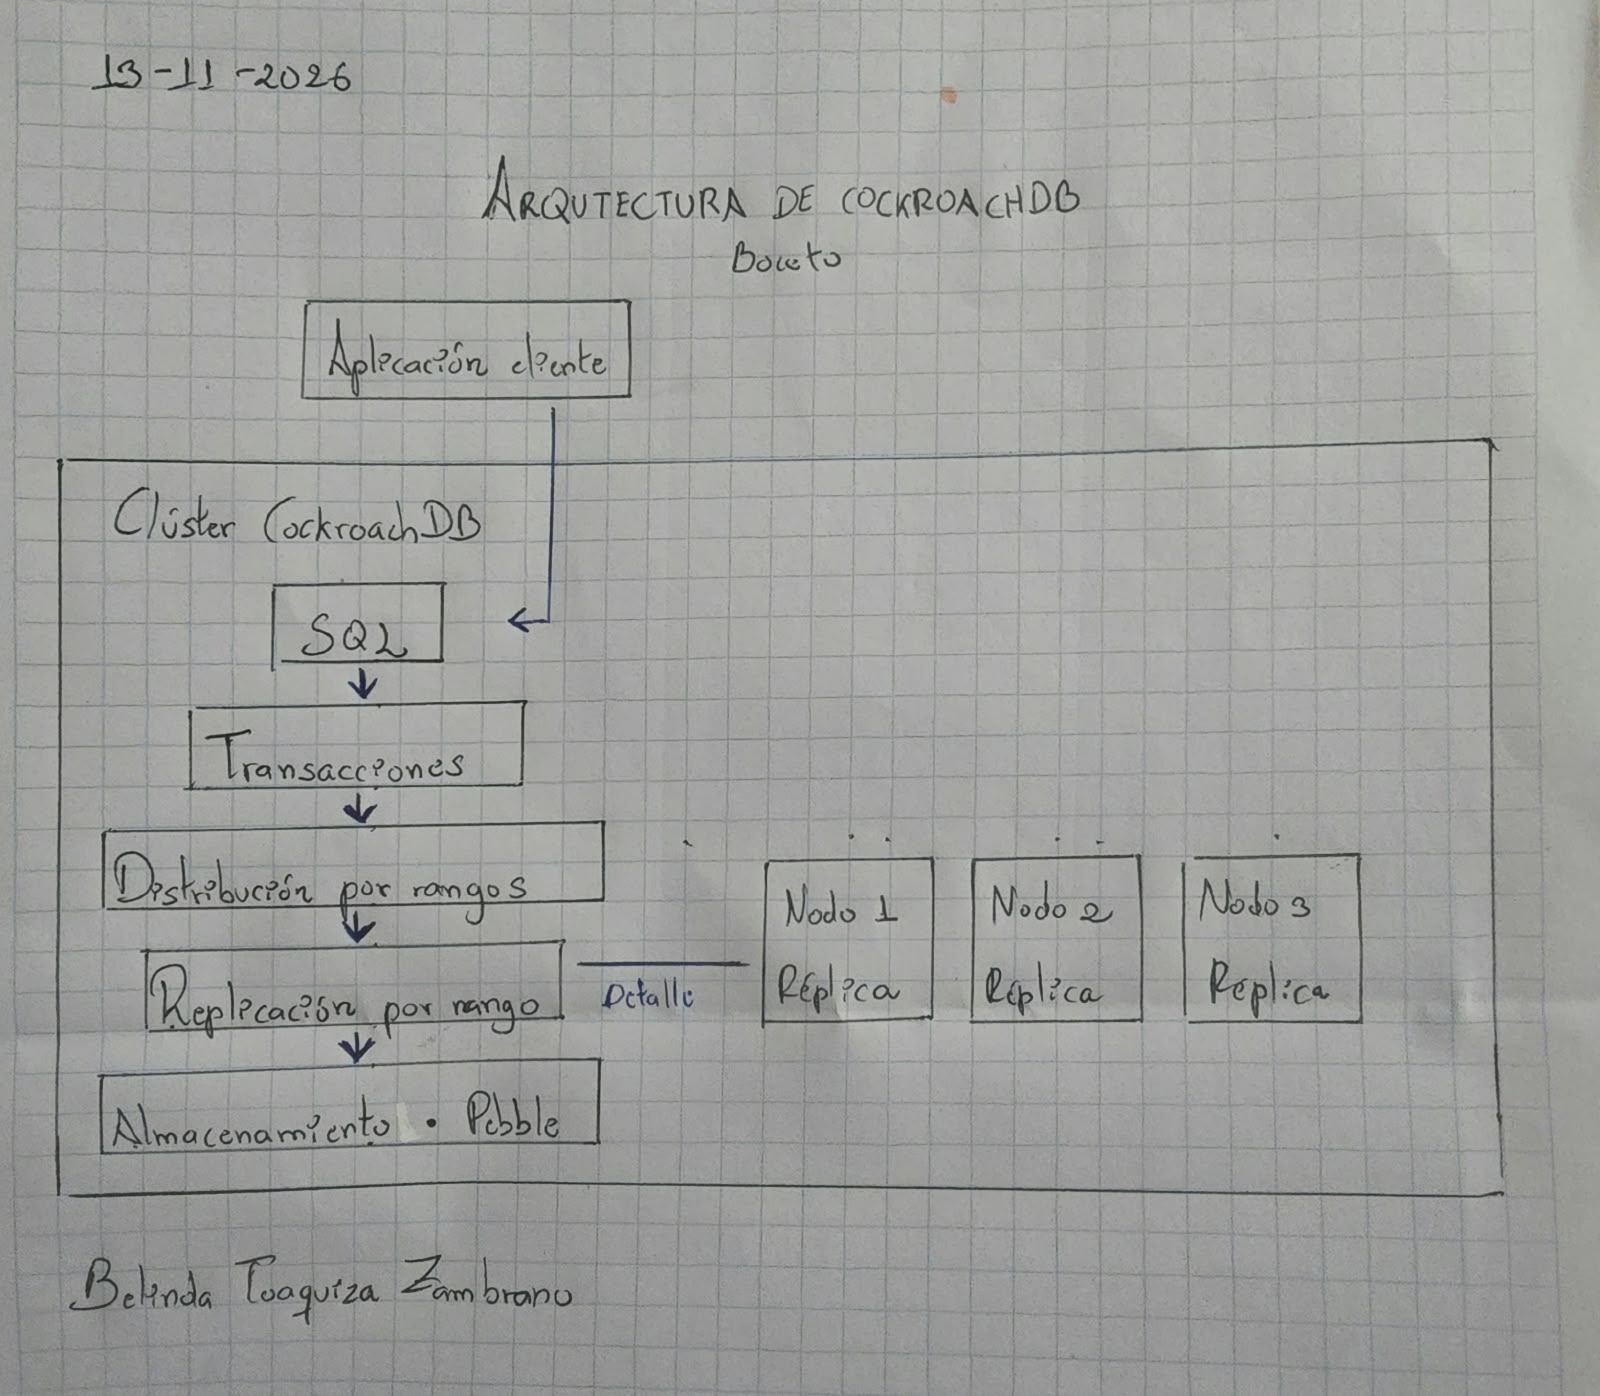
\includegraphics[width=0.85\textwidth]{figuras/esquema-a-mano.jpeg}
  \caption{Esquema inicial de la arquitectura de \sistemaA{}, dibujado a mano.}
  \label{fig:esquema-mano}
\end{figure}

\clearpage
\section*{Anexo B. Capturas de lectura de las fuentes}
\addcontentsline{toc}{section}{Anexo B. Capturas de lectura de las fuentes}
% Capturas de los artículos citados en la sección 3, con el fragmento utilizado
% subrayado en rojo y la página visible. Cada captura corresponde a una cita.
En cada captura se subrayó el pasaje empleado en la sección~3 y se indican el
número de la referencia y la página.

\begin{figure}[H]
  \centering
  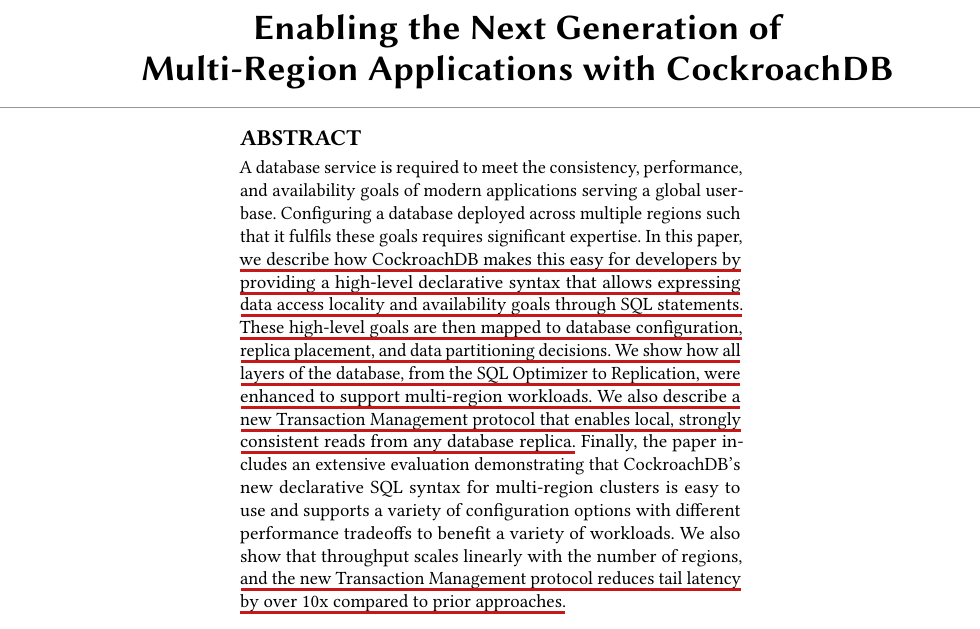
\includegraphics[width=0.92\textwidth]{Capturas/fuentes/fuente_01_vanbenschoten2022_multiregion_p01_subrayado.png}
  \caption{Fuente citada \cite{vanbenschoten2022multiregion}, p.~1: se subrayó la descripción de la sintaxis declarativa que expresa objetivos de localidad y disponibilidad de los datos y la del protocolo de transacciones que habilita lecturas locales fuertemente consistentes desde cualquier réplica; ambos pasajes sostienen la afirmación de la sección~3.2 sobre configuraciones de localidad y lecturas locales en despliegues multirregión.}
  \label{fig:lectura1}
\end{figure}

\begin{figure}[H]
  \centering
  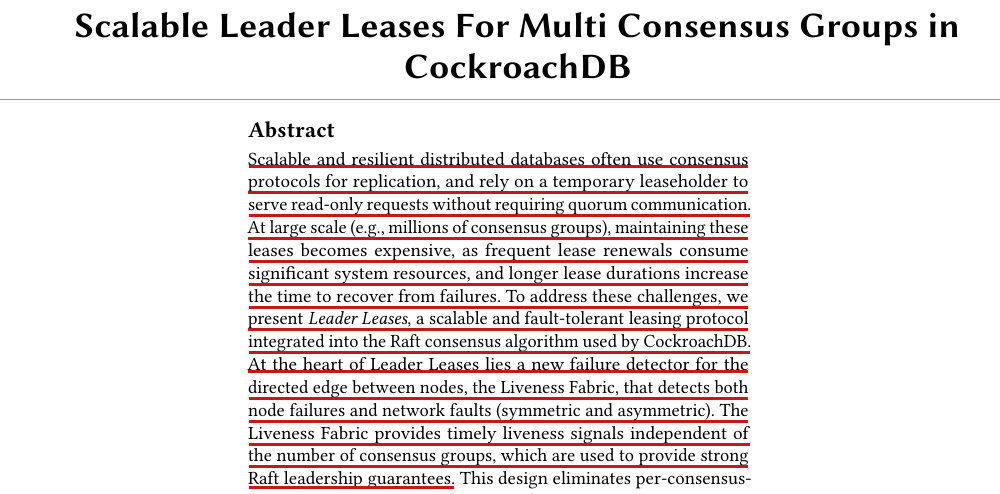
\includegraphics[width=0.92\textwidth]{Capturas/fuentes/fuente_02_kettaneh2026_leaderleases_p01_subrayado.png}
  \caption{Fuente citada \cite{kettaneh2026leaderleases}, p.~1: se subrayó la presentación del mecanismo Leader Leases, su integración en el algoritmo de consenso Raft y el detector distribuido de fallos Liveness Fabric; respalda lo expuesto en las secciones 3.3 y 3.4 sobre el arrendamiento del líder y su detección de vitalidad entre nodos.}
  \label{fig:lectura2}
\end{figure}

\begin{figure}[H]
  \centering
  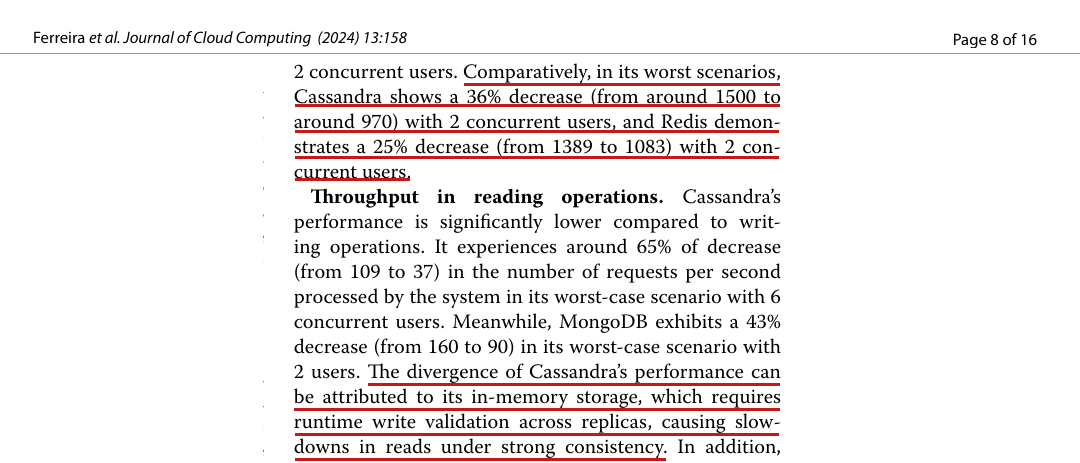
\includegraphics[width=0.98\textwidth]{Capturas/fuentes/fuente_03_ferreira2024_resultados_single_region_p08_subrayado.png}
  \caption{Fuente citada \cite{ferreira2024consistency}, p.~8: se subrayó el resultado que atribuye a Cassandra una caída del 36\,\% en el rendimiento de escritura y la explicación de la validación de escritura entre réplicas como causa de las lecturas lentas con consistencia fuerte; sustenta la afirmación de la sección~3.2 sobre diferencias de rendimiento asociadas a la configuración de consistencia.}
  \label{fig:lectura3}
\end{figure}

\begin{figure}[H]
  \centering
  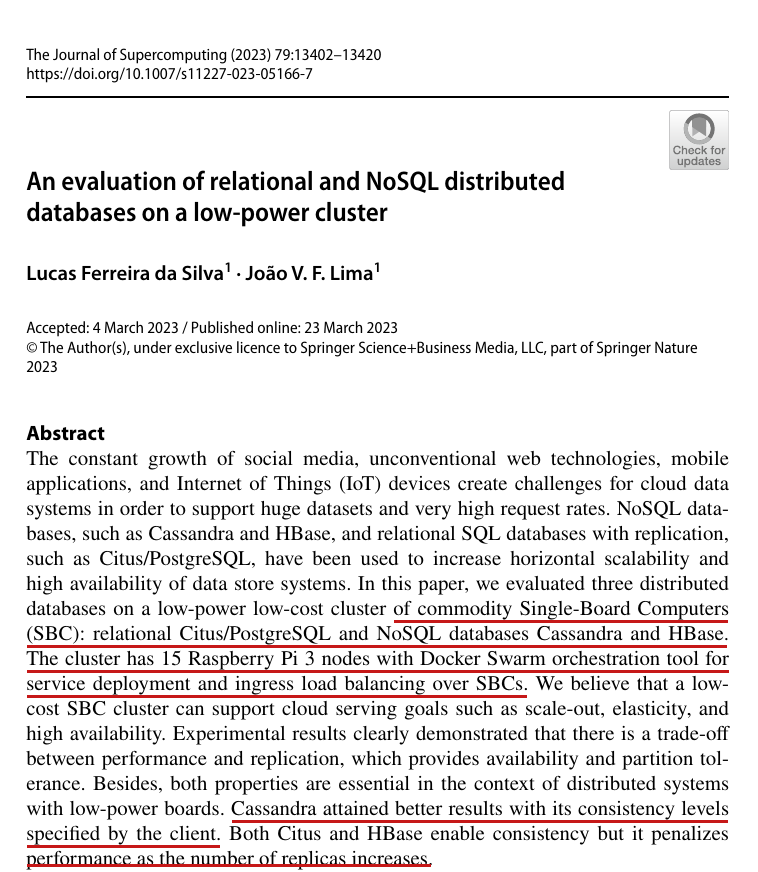
\includegraphics[width=0.62\textwidth]{Capturas/fuentes/fuente_04_silva2023_resumen_p01_subrayado.png}
  \caption{Fuente citada \cite{silva2023lowpower}, p.~1: se subrayó la evaluación de tres bases de datos distribuidas en un clúster de placas de bajo consumo con Docker Swarm y el resultado de Cassandra con los niveles de consistencia fijados por el cliente; respalda la mención de la sección~3.2 al clúster de placas de bajo consumo.}
  \label{fig:lectura4}
\end{figure}

\begin{figure}[H]
  \centering
  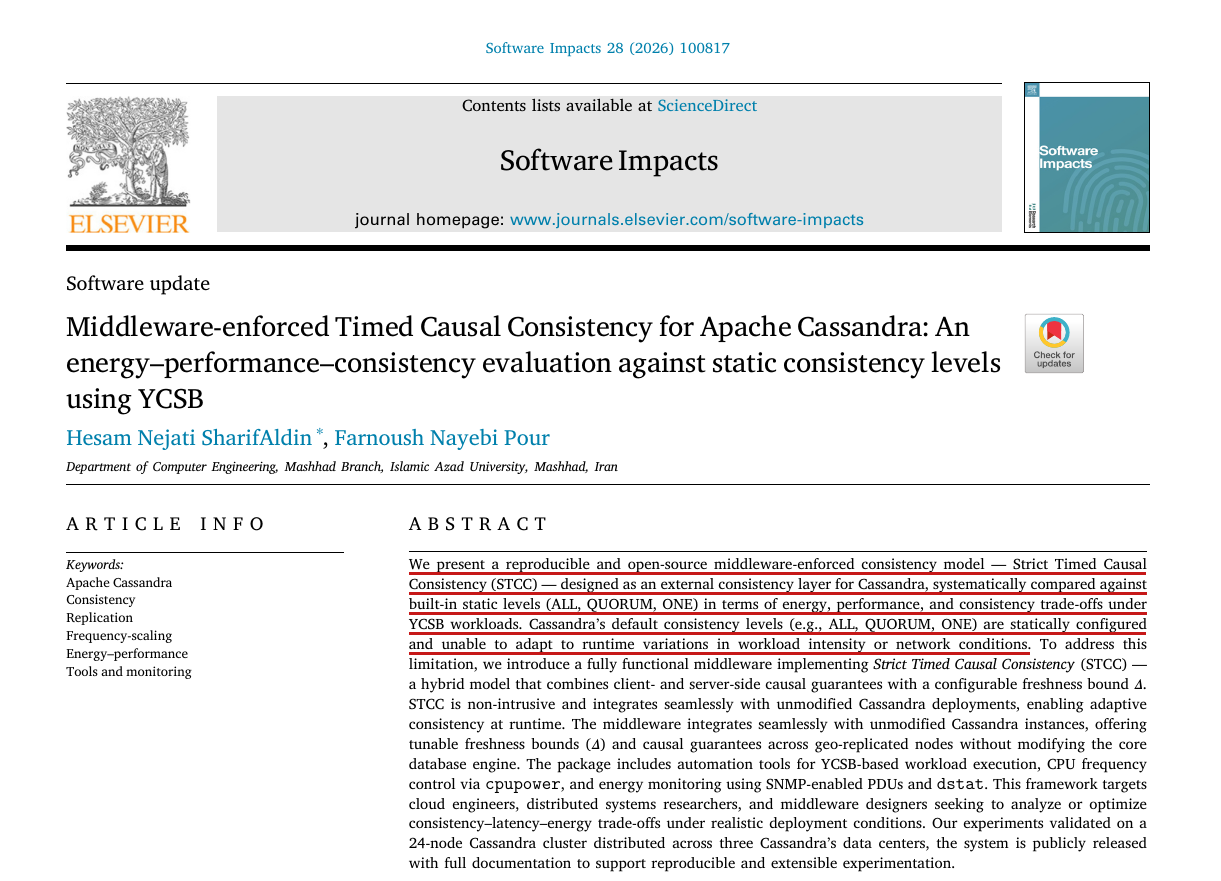
\includegraphics[width=0.98\textwidth]{Capturas/fuentes/fuente_05_nejati2026_abstract_p01_subrayado.png}
  \caption{Fuente citada \cite{nejati2026cassandra}, p.~1: se subrayó la presentación de STCC como capa de consistencia externa comparada con los niveles nativos de Cassandra y la descripción de esos niveles como estáticos; sustenta la afirmación de la sección~3.2 sobre la comparación con un middleware causal externo.}
  \label{fig:lectura5}
\end{figure}

\end{document}